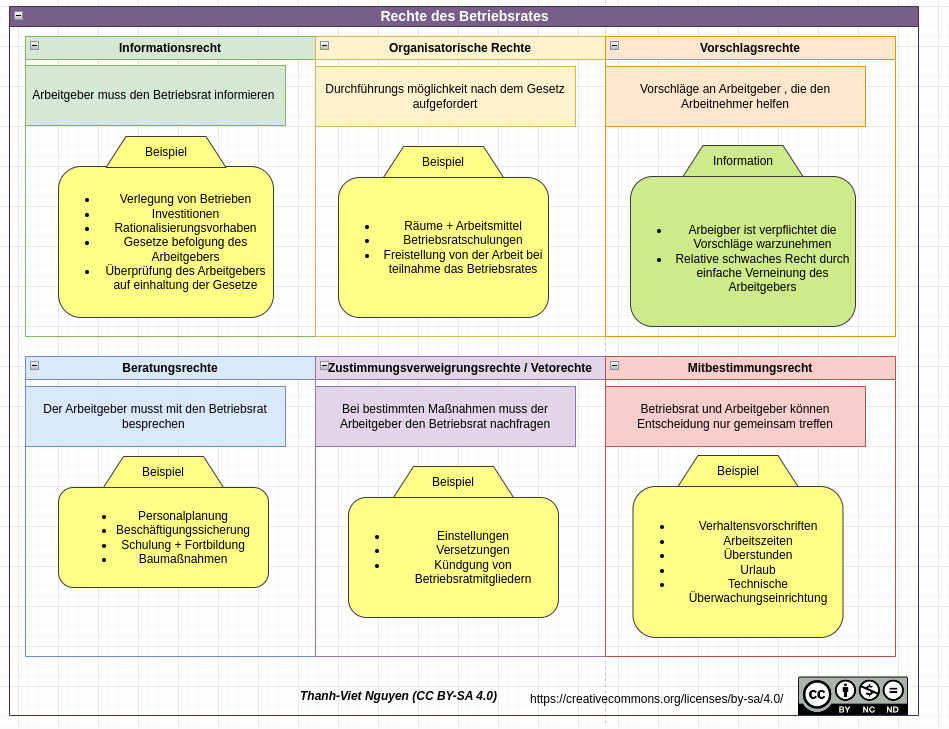
\includegraphics [width=15cm, height=10cm] {img/BetriebsratsRechte.png}
\begin{comment}
\begin{enumerate}
	\item 
	Informationsrechte
	\item 
	Vorschlagsrechte
	\item
	Beratungsrechte
	\item
	Zustimmungsverweigerungsrechte
	\item
	Mitbestimmungsrechte
	\item
	Organisatorische Rechte
	\item
	Sonstige Rechte
	\item
	Informations- und Unterrichtungsrechte
	\item
	Vorschlagsrechte
	\item
	Beratungsrechte
	\item
	Zustimmungsverweigerungsrechte
	\item
	Mitbestimmungsrechte
	\item
	Organisatorische Rechte
	\item
	Sonstige Rechte
	\item
	Rechte bei der Kündigung eines Arbeitnehmers
	\item
	Recht auf Einhaltung einer Betriebsvereinbarung oder Regelungsabrede
	\item
	Recht auf Einhaltung eines Einigungsstellenspruchs
	\item
	Unterlassungsanspruch bei Störung oder Behinderung der Betriebsratsarbeit
	\item
	Rechte bei groben Verstößen des Arbeitgebers (§ 23 Abs. 3 BetrVG)
	\item
	Recht auf Entfernung betriebsstörender Arbeitnehmer
	\item
	Hinzuziehungs- und Teilnahmerechte
\end{enumerate}
\end{comment}
